\section{Micro-Frontend Architecture}

Micro-frontends should bring the same advantages of microservices from the backend to the frontend. Instead of creating a large frontend monolith, a micro-frontend architecture contains many small applications. The advantage is that every micro-frontend can be developed and deployed by a separate team. \cite{book:2020:geers:background:micro-frontends:micro-frontends-in-action} The difference between frontend-monoliths and micro-frontends can be seen in figure \ref{figure:state-of-the-art:ui-monolith-micro-frontend}.

\ifshowImages
\begin{figure}[H]
\centering
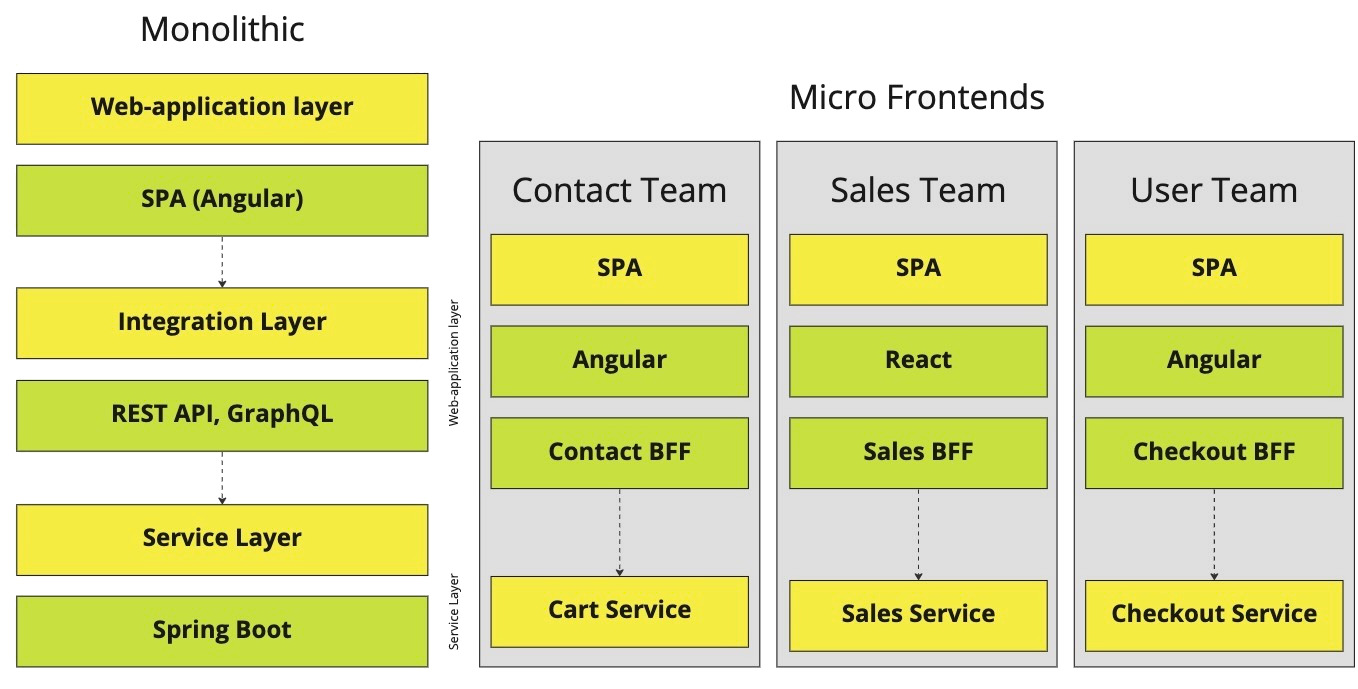
\includegraphics[width=0.8\linewidth]{images/ui-monolith-micro-frontends.jpeg}
\caption{A comparison between frontend-monoliths and micro-frontends.}\label{figure:state-of-the-art:ui-monolith-micro-frontend}
\end{figure}
\fi

Benefits gained from working with microservices on the backend are lost, when working with a monolithical frontend. With a monolithic frontend, the ability to deploy independently is lost. The entire frontend has to be deployed at once. Another problem is, that distinct operations are not really possible. If one part of the frontend is broken, there is a good chance that the entire frontend is broken. Another problem is the parallel development. The speed of development cannot be increased because it is very difficult to have multiple teams working on one frontend application. \cite{misc:2019:leitner:micro-frontends}

The term micro-frontend can be misleading, as can the term microservice. It has no meaning in terms of the size of the application. It can be a simple widget that only displays data, or a full-blown one-page application. Ideally, a micro frontend covers an area of the entire frontend application.


Micro-frontends try to apply the same principles from the microservice architecture to frontend development. Often times a microservice architecture with is developed by several teams has only one frontend application. Therefore, when adding new features a single team can be overwhelmed. Like a microservice architecture, a micro-frontend architecture focuses on developing many small frontend-applications, instead of developing a large software monolith. Each micro-frontend can be developed independently by another team. But a challenge is that the micro-frontend should appear as a single application to the user. Therefore, the different applications have to be integrated, which can be a challenge.

The term micro-frontend should not lead to false conclusions about the size of an application. The size of micro-frontends can vary. It can range from a simple login to a complex single-page application.

Building micro-frontends with the web allows different strategies of integrating the applications. Three different strategies exist to combine multiple micro-frontends into an app-shell. The client-side integration, the server-side integration and the combination of these two strategies and the combination of both strategies.

\subsection{Characteristics}

Micro-frontends tend to follow the same characteristics as microservices.

\subsubsection{Autonomous}

Technically a micro-frontend is a completely independent and runnable application. The integration of the micro-frontends happens only through the frontend. The different micro-frontends are composed withing an app-shell. The application shell is a separate application that is usually the entry-point for the user to interact with all micro-frontends. The app-shell also provides the layout of the page and defines where the micro-frontends are placed. The autonomy should not go in the direction of complete isolation. But no dependencies should emerge, which could the autonomy. \cite{book:2020:geers:background:micro-frontends:micro-frontends-in-action}

\subsubsection{Technology Agnostic}

Just as microservices architectures, micro-frontend architectures can be technology agnostic. The current frontend development landscape offers a lot of JavaScript frameworks to choose from. The advantage of an application that consists of small independent building blocks is that parts can be rewritten with another technology more easily. \cite{book:2020:geers:background:micro-frontends:micro-frontends-in-action} But using different technologies for different micro-frontends can lead to problems with the chosen form of integration and communication. The communication should be technology agnostic as well and should use browser native tools like Broadcast API.

Another problem that could arise is the bundle size of modern JavaScript frameworks. If two frameworks like React and Angular need to be fetched, the total bundle size can be very large and a strain for network connections. Loading an running multiple micro-frontends is also resource intensive. Due bypass this problem and offer a standardized API, micro-frontends can be developed with the help of Web Components. With this approach, no specific framework is needed to the application. \cite{book:2020:geers:background:micro-frontends:micro-frontends-in-action} 

\subsubsection{Independently Depoyable}

The autonomy of micro-frontends offer the possibility for independent deployments. A large monolithical frontend application is more complex to deploy. There is no need to have communication and coordination over multiple teams to deploy the application. Organizational dependencies have a negative impact on the time-to-market, because development teams would have to wait for the release of another team. \cite{book:2020:geers:background:micro-frontends:micro-frontends-in-action} 

\subsubsection{Small and Easy to Maintain}

Because micro-frontends only cover a small domain of an application, the source code is smaller and easier to understand. A smaller codebase is especially helpful for understanding the inner workings of software. 
Due to the easier understanding of the domain, the application can be easier rewritten with a state of the art technology, if the old one becomes deprecated. \cite{book:2020:geers:background:micro-frontends:micro-frontends-in-action}

\subsubsection{Resilience}

Micro-frontends offer the possibility to build an application by composing multiple independent applications into a fully fledged application. Depending on the integration strategy micro-frontends are usually combined at runtime. But the network, especially for mobile devices is not always without failures. A micro-frontend architecture provide better failure isolation. One micro-frontend crashing does not have an effect on the other micro-frontends inside the application. Some parts of the application might not work, but other parts of the application are still useable. The app-shell can react to a failure and tell users that the application is not working as expected and will be available back soon. \cite{article:2021:perltonen:background:micro-frontends:motivations-benefits-and-issues}

\subsection{Downsides of Micro-frontend architecture}

Due to the many advantages of micro-frontends there are also a downsides using this architectural approach. The independent development comes with the disadvantage of having redundancies. Each micro-frontend needs a separate build-process and also a continuous integration pipeline. And if the backend-for-frontend approach is, every micro-frontend needs it own backend-for-frontend service. It might happen that a lot of code is duplicated. when implementing this pattern. If multiple teams use the same code and a bug is found, the wrong behavior can't be fixed in a central place. Therefore, it is important to share knowledge between the teams to avoid running in the same bad situations over and over again. But this should not lead to inter-team dependencies between the different teams.
\cite{book:2020:geers:background:micro-frontends:micro-frontends-in-action} 


\subsection{Integration strategies}\label{subsection:background:micro-frontend-architecture:integration-strategies}

Micro-frontends can be integrated with different strategies. The integration strategy depends on the requirements of the system. They can be composed using a client-side integration strategy, a server-side strategy, or a combination of both.

\subsubsection{Server-Side Integration}\label{subsubsection:background:micro-frontend-architecture:integration-strategies:server-side-integration}

A Service between the client and the backend usually does server-side composition. \cite[60]{book:2020:geers:background:micro-frontends:micro-frontends-in-action} The server responds with references to micro-frontends that should be included and their required assets. The service in the middle intercepts that response and replaces the references to the micro-frontends with the actual content before the response is sent to the browser. The micro-frontends are included in their position and later appear in the HTML. An example of a server-side include can be seen in listing \ref{code:background:micro-frontends:server-side-include}. The other micro-frontends are referenced with URLs. \cite[61-63]{book:2020:geers:background:micro-frontends:micro-frontends-in-action}

\ifshowListings
\begin{listing}[H]
    \begin{minted}{html}
<html>
  <body>
    <!--#include virtual="/erp/dashboard" -->
  </body>
</html>
    \end{minted}
    \caption{An example server-side include.}\label{code:background:micro-frontends:server-side-include}
\end{listing}
\fi

\bigskip

\noindent One advantage of server-side integration is the fast first-load performance, which is the principle of progressive enhancement. \cite{book:2010:parker:background:micro-frontends:designing-with-progressive-enhancement} The browser fetches the HTML and renders it. It does not have to assemble parts of a page, like with client-side integration. The computation is only done on the server, which reduces the strain on the user's device. \cite{book:2020:geers:background:micro-frontends:micro-frontends-in-action} However, assets like stylesheets and images must still be fetched from the server. Server Side Integration is helpful if the application's primary concern is presenting static content to the end user and instant reaction to the users' inputs is unnecessary.  \cite[83]{book:2020:geers:background:micro-frontends:micro-frontends-in-action}

\subsubsection{Client-Side Integration}\label{subsubsection:background:micro-frontend-architecture:integration-strategies:client-side-integration}

When the application should react promptly to user input, a client-side integration strategy is preferred. For example, when developing an online marketplace, the user should be able to add items to the cart without making a complete roundtrip to the server to see the updated value. The application should provide a seamless user experience, as the end user just uses one application. Modern Frameworks like Angular and React offer the development of Single Page Applications, which provide reactive, client-side rendered applications. The HTML Markup is produced on the client instead of the server. \cite{book:2020:geers:background:micro-frontends:micro-frontends-in-action}

\bigskip

\noindent Client-side integration can be achieved through different approaches. The most straightforward approach combines the micro-frontends by linking the different applications with Hyperlinks. Each micro-frontend is deployed and accessible via a different URL, and the different micro-frontend applications are then linked with Hyperlinks. As the approach implies, switching to another micro-frontend requires a complete page reload and a roundtrip to the server. However, the integration with Hyperlinks breaks the SPA approach. This strategy makes it necessary that every micro-frontend is accessible via its URL and that it can be served as a standalone application.

\bigskip

\noindent Another client-side approach is to combine micro-frontend with iFrames or Web-Components. Integrating micro-frontends with this approach enables the page to be a SPA still. The client can navigate multiple micro-frontends without noticing, and no page reloads are needed. An iFrame is an isolated area with its own browser context \cite[35]{book:2020:geers:background:micro-frontends:micro-frontends-in-action}, Web Components are self-created HTML elements that are embedded into the DOM of the browser \cite[103]{book:2019:farrell:background:micro-frontends:web-components-in-action}. Integrating applications with the client-side strategy using Module Federation is explained in more detail in section \ref{subsubsection:background:micro-frontend:module-federation:101}.


\subsection{Communication between Micro-frontends}

Micro-frontends should not depend on each other. But it is necessary to have communication between them. For example if a user adds an item to a shopping-cart in an e-commerce application, the product micro-frontend has to inform the shopping-cart micro-frontend, which item was added. To reduce the coupling between applications and development teams it is recommended to keep the communication between micro-frontends at a minimum. Before choosing a communication pattern it is important to know the type of communication. If communication between two micro-frontends or between the app shell and a micro-frontend is required, the communication can take place via the user interface. Other communication mechanisms, like the Broadcast Channel API provided by the browser, are useful for state sharing or for passing on information to multiple micro-frontends. \cite{book:2020:geers:background:micro-frontends:micro-frontends-in-action}

\bigskip

\noindent When the micro-frontends are integrated via hyperlinks, the communication can only happen via URL parameters. Single-Page-Applications usually communicate via custom events and attribute changes of the components. \cite[100]{book:2020:geers:background:micro-frontends:micro-frontends-in-action} \cite[315-316]{book:2019:farrell:background:micro-frontends:web-components-in-action} A distinction can be made between \textbf{parent-to-fragment}, \textbf{fragment-to-parent} or \textbf{fragment-to-fragment} communication, where the term fragment is equivalent to a micro-frontend and the term parent is equivalent to the app shell. \cite{book:2020:geers:background:micro-frontends:micro-frontends-in-action} This is further shown in figure \ref{fig:background:micro-frontend:communication:communication-patterns}

\ifshowImages
\begin{figure}[H]
    \centering
    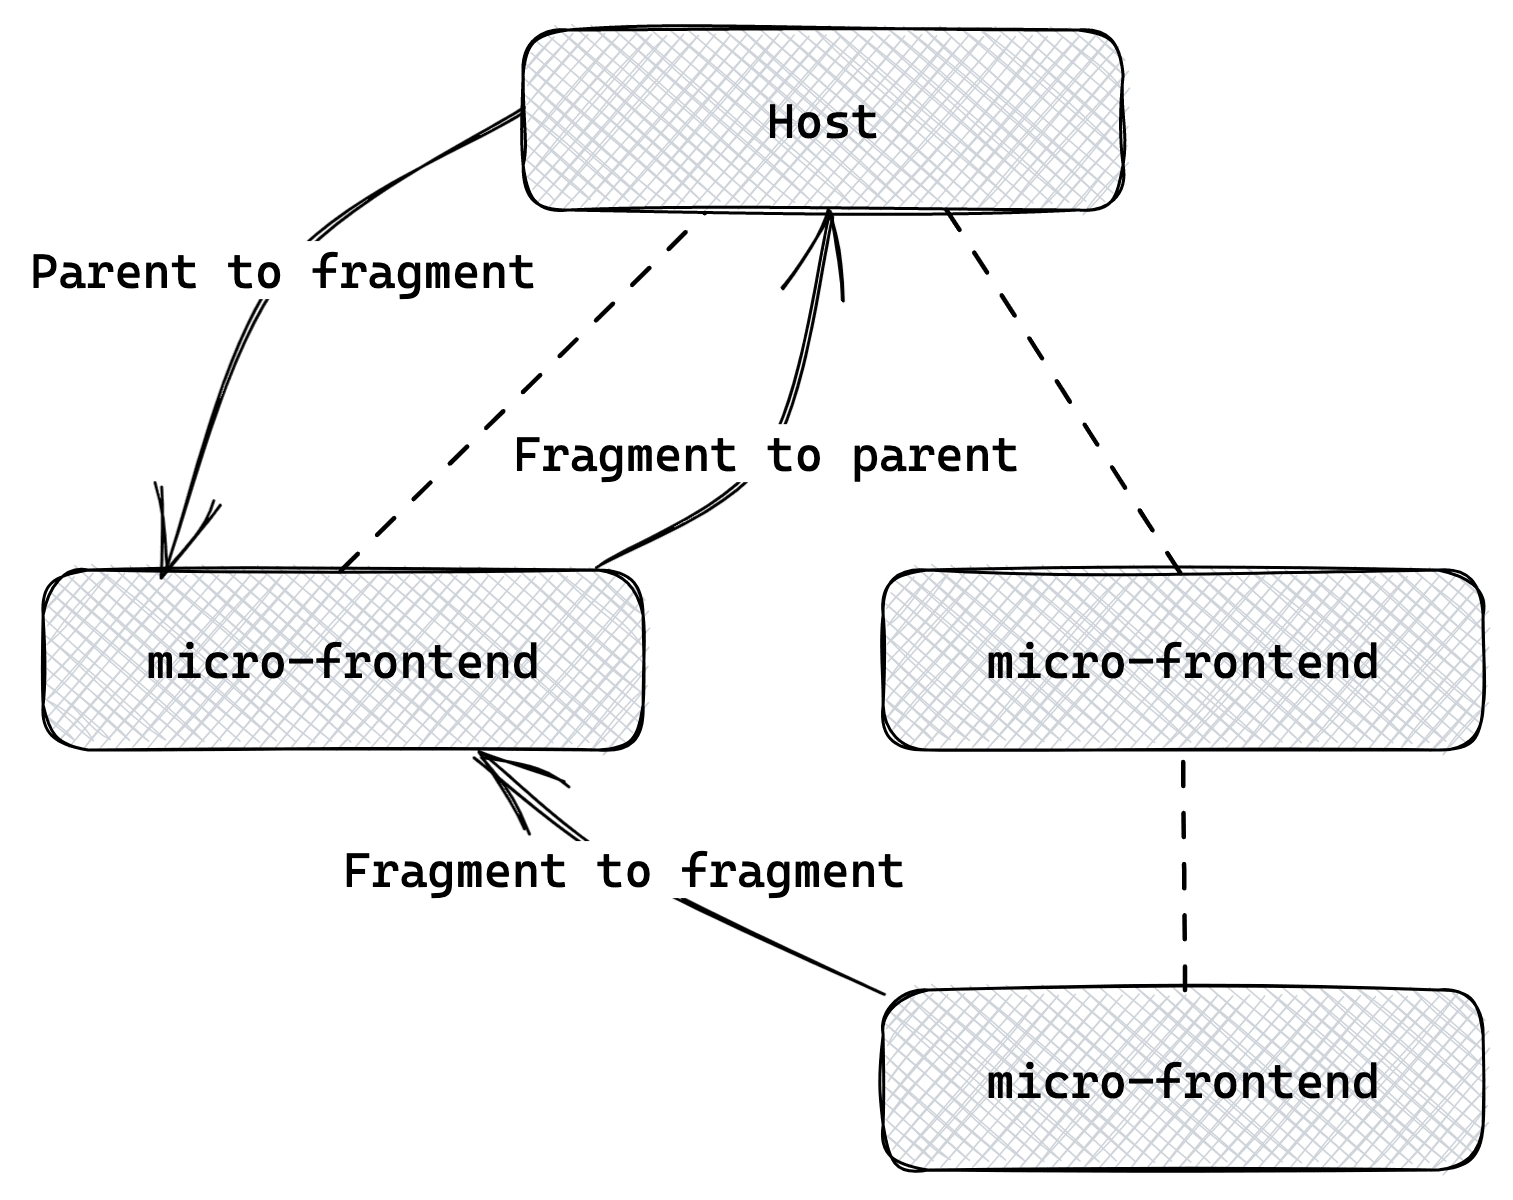
\includegraphics[width=0.5\linewidth]{images/background/communication/communication-patterns.png}
    \caption{Different forms of communication in micro-frontend architectures (Adapted from \cite[100]{book:2020:geers:background:micro-frontends:micro-frontends-in-action})}\label{fig:background:micro-frontend:communication:communication-patterns}
\end{figure}
\fi

\bigskip

\noindent Parent-to-fragment communication can happen via attribute changes when using Web Components. \cite[58-59]{book:2019:farrell:background:micro-frontends:web-components-in-action} To pass data from a micro-frontend to the app shell, custom-events can be used. \cite[315]{book:2019:farrell:background:micro-frontends:web-components-in-action}, where the micro-frontend emits an event, that the app shell is subscribed to. \cite{book:2020:geers:background:micro-frontends:micro-frontends-in-action}

\bigskip

\noindent Fragment-to-fragment communication is required when two micro-frontends should communicate with each other. The changes of one micro-frontend should have an effect on the other micro-frontend. This form of communication can be implemented in three ways: \cite[107-108]{book:2020:geers:background:micro-frontends:micro-frontends-in-action}

\begin{itemize}
    \item \textbf{Direct communication}: This is the most direct form of communication. One micro-frontend changes the attributes of its HTML elements with JavaScript. This approach is not recommended, because it introduces high coupling between two micro-frontends. One micro-frontends needs to know implementation details of the other micro-frontend. This makes it difficult to change the implementation of one micro-frontend without breaking the other micro-frontend. And this breaks one characteristics of micro-frontends, which are independent and autonomous development and deployment.
    \item \textbf{Orchestration via a parent}: When using this approach, the app shell is responsible for the communication between micro-frontends. One micro-frontend emits an event, which is intercepted by the app-shell. The app-shell sends the event to the target micro-frontend. This approach allows the micro-frontends to be completely decoupled, but changes have to be adapted by every micro-frontend.
    \item \textbf{Event-Bus/broadcasting}: Instead of a direct communication between micro-frontends or an indirect communication via the app-shell, a micro-frontend can publish an event on a central event-bus. The other micro-frontends can subscribe to the event and react to it. This is described as publish/subscribe mechanism. This drastically reduces the coupling between micro-frontends. No micro-frontend needs any information about the other micro-frontends, which allows perfect parallel development.
\end{itemize}


\subsection{Generic APIs vs Consumer Driven APIs}\label{subsection:background:micro-frontend:generic-vs-consumer-driven-apis}

The big decision in micro-frontend \ac{API} development is to use either generic or consumer-oriented \acp{API}. The difference is that generic \acp{API} emphasize reusability, while consumer-oriented \acp{API} tailor the \acp{API} to the customer.

\subsubsection{Generic \acp{API}}\label{subsubsection:background:micro-frontend:generic-vs-consumer-driven-apis:generic-apis}

Generic \acp{API} refer to \acp{API} that are very general and can be used by different clients. However, this type of \ac{API} has two significant drawbacks. Over-fetching describes the problem of getting more data than is needed, and Over-requesting describes the problem of needing multiple requests to get the data for a use case. Both problems are discussed in more detail in the following paragraphs. \cite{misc:2019:leitner:background:micro-frontends:backend-for-frontends}

\paragraph{Over-Fetching}\label{paragraph:background:micro-frontend:generic-vs-consumer-driven-apis:generic-apis:over-fetching}


For example, a contact service provides a contact model that includes \texttt{customerNumber}, \texttt{firstName}, \texttt{secondName}, \texttt{uidNumber}, and the user's address, as seen in the listing \ref{code:background:micro-frontends:over-fetching}. However, one application requirement is to display only a contact's first and last name inside the header. Only two fields of the model are used, and the rest are unnecessarily queried. \cite{misc:2019:leitner:background:micro-frontends:backend-for-frontends}

\ifshowListings
\begin{listing}[H]
    \begin{minted}{typescript}
interface ContactModel {
  id: string;
  customerNumber: string;
  firstName: string;
  secondName: string;
  uidNumber: string;

  Address: {
    id: string;
    postalCode: string;
    location: string;
    Country: string;
  }
}
    \end{minted}
    \caption{Contact-Model that contains too many fields for the requirement.}\label{code:background:micro-frontends:over-fetching}
\end{listing}
\fi

\paragraph{Over-Requesting}\label{paragraph:background:micro-frontend:generic-vs-consumer-driven-apis:generic-apis:over-requesting}

Attempting to solve the problem of over-fetching by reducing the amount of data set that is returned leads directly to this problem. Listing \ref{code:background:micro-frontends:over-requesting} shows the problem of over-requesting. If another requirement inside the application should display the address alongside the contact, two requests have to be performed every time. Afterwards, the two data sets have to be merged, leading to high client complexity. \cite{misc:2019:leitner:background:micro-frontends:backend-for-frontends}

\ifshowListings
\begin{listing}[H]
    \begin{minted}{typescript}
interface ContactModel {
  id: string;
  customerNumber: string;
  firstName: string;
  secondName: string;
  uidNumber: string;

  address_id: string;
}
    \end{minted}
    \caption{Contact-Model model that links the address-model with an id.}\label{code:background:micro-frontends:over-requesting}
\end{listing}
\fi

\subsubsection{Consumer Driven \acp{API}}\label{subsubection:background:micro-frontend:generic-vs-consumer-driven-apis:consumer-driven-apis}

Consumer-driven \acp{API} are the opposite of generic \acp{API}. They follow the idea of providing the client with exactly the data it needs. Following the example above, the contact service would have an endpoint that returns only the first and last name as required for the request. These endpoints make communication with a client straightforward, and there is no problem of over-fetching and over-requesting. However, creating an endpoint for each request creates an unmanageable set of endpoints.  \cite{misc:2019:leitner:background:micro-frontends:backend-for-frontends} To solve the problems of Over-fetching and Over-requesting, the \ac{BFF} pattern is often used. This pattern provides each client with their own \ac{API}, which is adapted to their needs. \cite{book:2018:richardson:background:bff:microservices-patterns}

\ifshowImages
\begin{figure}[H]
    \centering
    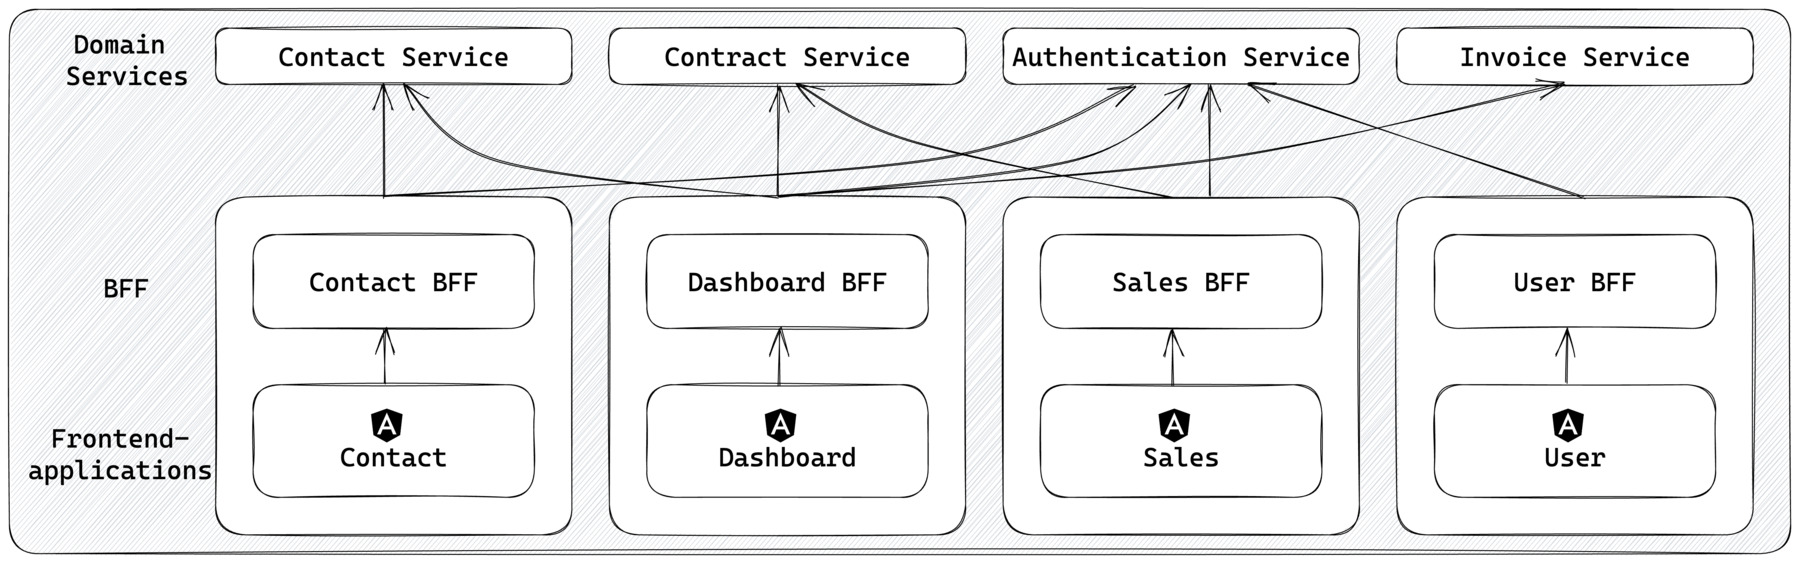
\includegraphics[width=1\linewidth]{images/background/micro-frontends/bff-architecture.jpg}
    \caption{Frontend architecture with the \ac{BFF} pattern.}\label{fig:background:micro-frontend:bff-architecture}
\end{figure}
\fi

\noindent Figure \ref{fig:background:micro-frontend:bff-architecture} shows an exemplary micro-frontend architecture using the \ac{BFF} pattern. Each frontend has a service that retrieves data only for that specific client. Because the \acp{BFF} function as a gateway to the domain services, the domain services can stay very generic and be reused by different clients. \acp{BFF} should implement only the presentation logic that puts the data into the form that the client needs, and it should avoid storing state. \cite{misc:2019:leitner:background:micro-frontends:backend-for-frontends}

\bigskip

\noindent With this architectural approach, the \ac{BFF} and the frontend form a single deployment unit. If one application changes, the other must adapt to the changes. GraphQL is a perfect technology for implementing a \ac{BFF} because it is specifically designed for implementing the presentation layer.
